\chapter{Dataset and evaluation metrics}
\label{Dataset}

In the first section (\ref{dataset}) we describe the dataset which is used for training and evaluation purpose for the task of the human pose estimation.
In the second (\ref{evaluation-metric}) section the define the evaluation metric for aforementioned

\section{Dataset}
The most common datasets for the task of human pose estimation from point clouds are ITOP \parencite{haque_towards_2016} and EVAL \parencite{liu_point_2020}. In this work we concentrate on ITOP dataset since it's more widely used thus has more related works for results' comparison.

\label{dataset}
\subsection{ITOP}

ITOP dataset was first released in the work of \cite{haque_towards_2016}. The dataset comprises depth images of people in different poses. In Figure~\ref{img:dataset-points-with-depth} are shown example of the depth map from the dataset. 

The snapshots of poses are taken from two different viewpoints: the front view, and the top view. In front view the camera faces a person directly in front (the whole body is seen). In top view the camera is placed above the person and shots the view from the top (torso usually occluded by shoulders and arms).

The dataset is collected inside of the room thus some furniture items appear in the dataset. Due to excess obstacles in the field of view of the camera, we apply preprocessing pipelines to extract only human point cloud. The pipeline is described in Section~\ref{Data-preparation}. Figures \ref{img:dataset-human-examples-front-view} and \ref{img:dataset-human-examples-top-view} show examples of font and top view respectively.

Ground truths consist of 15 joint key points - head, neck, shoulders, elbows, hands, torso, hips, knees, and foots. An example of named joints is shown in Figure~\ref{img:dataset-example-joints}. Table~\ref{tab:dataset-statistic} covers general statistics on dataset size.

\begin{table}
    \label{tab:dataset-statistics}
    \caption{General statistic for ITOP dataset}
    \centering
    \begin{tabular}{l l l l}
    \toprule
    \tabhead{View} & \tabhead{Split} & \tabhead{Frames} & \tabhead{People} \\
    \midrule
        side & train & 39,795 & 16 \\
        side & test  & 10,501 & 4  \\
        top  & train & 39,795 & 16 \\
        top  & test  & 10,501 & 4  \\
    \bottomrule\\
    \end{tabular}
\end{table}

\begin{figure}[htbp]
    \centerline{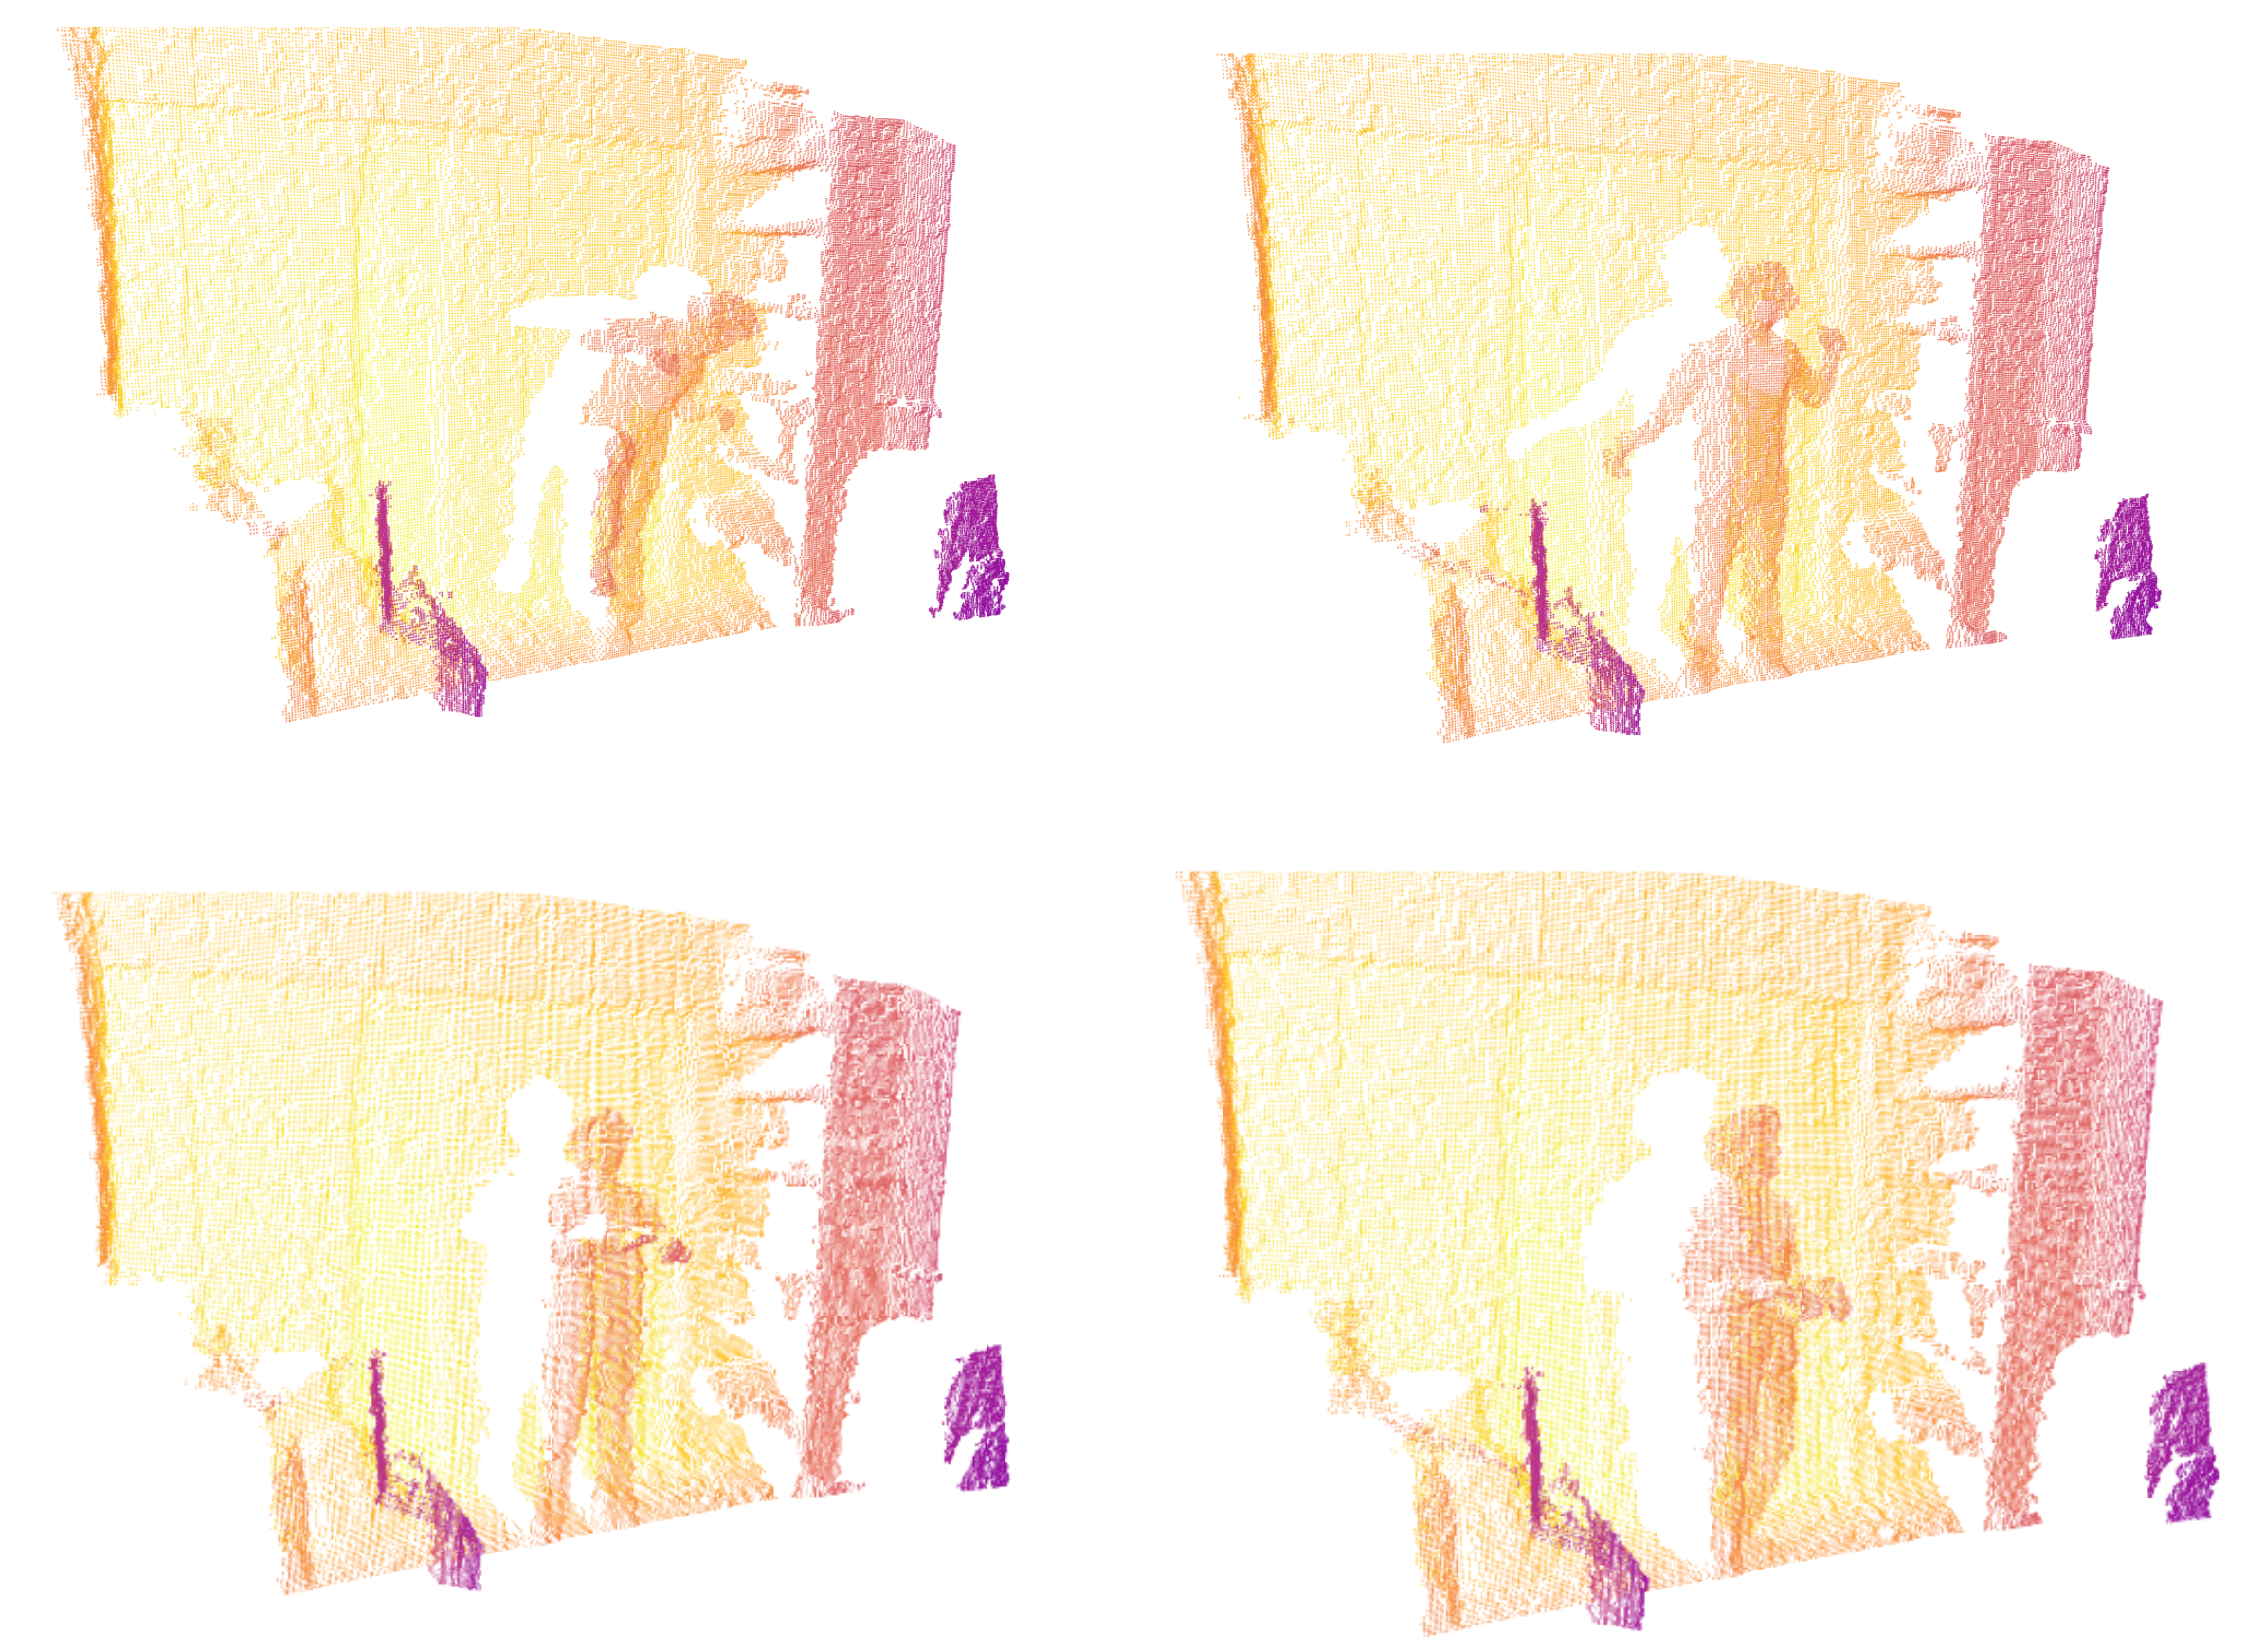
\includegraphics[scale=.17]{Figures/points-with-depth.png}}
    \caption{Four examples of depth images from ITOP dataset. The darker the color the closer it's located to the camera}
    \label{img:dataset-points-with-depth}
\end{figure}

\begin{figure}[htbp]
    \centerline{\includegraphics[scale=.15]{Figures/dataset examples - side view.png}}
    \caption{Four examples of front view subset of ITOP. Upper images are depth representation. Bottom images show human point clouds (blue) with key joints (red)}
    \label{img:dataset-human-examples-front-view}
\end{figure}

\begin{figure}[htbp]
    \centerline{\includegraphics[scale=.15]{Figures/dataset examples - top view.png}}
    \caption{Four examples of top view subset of ITOP. Upper images are depth representation. Bottom images show human point clouds (blue) with key joints (red)}
    \label{img:dataset-human-examples-top-view}
\end{figure}

\begin{figure}[htbp]
    \centerline{\includegraphics[scale=0.8]{Figures/dataset-example-joints.png}}
    \caption{Example of key joints with names from ITOP dataset}
    \label{img:dataset-example-joints}
\end{figure}

\section{Evaluation metric}
\label{evaluation-metric}
Since we are working on the task of the regression, we use mean Average Precision (mAP) as our main metric of model's performance. The ground truths are coordinates of key human joints (denoted as $J$). The output of the regression model is also joints' coordinates of the same size as $J$ (denoted as $\hat{J}$).

To be able to compare our results with other works \parencite{haque_towards_2016,moon_v2v-posenet_2018,guo_towards_2017} we use the same approach of calculation of $AP$ using $10 \ cm$ distance threshold. By this rule (Formula~\ref{eqn:dataset-metric-ap}) the predicted joint is considered correctly detected if the $L_2$ distance to ground truth is equal or less that $10 \ cm$. The resulting $mAP$ is calculated by averaging $AP$ by the number of samples (Formula~\ref{eqn:dataset-metric-map}).

For further convenience we will also apply the plot with $mAP$ values for distances from $0 \ cm$ to $100 \ cm$ (Example in Figure~\ref{img:example-map}).

\begin{equation}
\label{eqn:dataset-metric-ap}
AP(J, \hat{J})=\left\{\begin{array}{ll}
    1, & \lVert J - \hat{J} \rVert <10 \mathrm{~cm} \\
    0, & \text { otherwise }
\end{array}\right.
\end{equation}

\begin{equation}
\label{eqn:dataset-metric-map}
    mAP=\frac{\sum_{i=0}^{M} A P\left(J_{i}, \hat{J_{i}}\right)}{M}
\end{equation}

\begin{figure}[htbp]
    \centerline{\includegraphics[scale=.6]{Figures/example-map.png}}
    \caption{Example of the mAP plot. On the X axis - allowed distance between predicted and ground truth coordinates to be considered as a right detection. On the Y axis - mean Average Precision for given distance. The values for $\textbf{distance} = 10 \ cm$ is highlighted on the plot.}
    \label{img:example-map}
\end{figure}